\documentclass[11pt]{article}
\usepackage{graphicx}
\usepackage[utf8]{inputenc}
\usepackage{geometry}
\usepackage{titlesec}
\usepackage{float}
\usepackage{enumitem}
\usepackage{hyperref} 
\usepackage{amsmath}
\usepackage{ gensymb }
\usepackage{ amssymb }
\usepackage{float}
\usepackage{amsthm}
\usepackage{float}
\usepackage{pgfplots}
\pgfplotsset{compat=1.17}

\newcommand{\st}{\text{s.t}}
\newcommand{\R}{\mathbb{R}}
\newcommand{\N}{\mathbb{N}}

\title{ECON 20110 PSET 2}
\author{Anthony Yoon}
\date{1/24/2025}
\begin{document}
\maketitle

\section*{1}
\subsection*{a}
Let $y_1$ denote cotton threads, such that $y_1 \in Y$. Let $x_1$ denote raw cottoon such that $x_1 \in C$ and $x_2 \in L$. Therefore we see that the production possibility set that describes Firm 1's technology is $F_1 \subseteq X \times Y$ where $F_1 = \{ (x_1, x_2, y_1) \in \R^2_+ \hspace{2pt} \}| \hspace{2pt} y_1 \leq x^{\frac{1}{2}}_1 x^{\frac{1}{2}}_2 \}$. 
\subsection*{b}
Let $y_1$ and $Y$ be denoted the same as before. Let $y_2 \in P$ where $y_2$ is the number of pillow cases and $P$ is the set of all pillow cases. Thus, the production possiblity set denoted by $F_2$ and is $F_2 \subseteq Y \times P$, where $F_2 = \{ (y_1, y_2) \in \R^2_+ \hspace{2pt} | \hspace{2pt} y_2 \leq y_1^{\frac{1}{2}}\}$. 
\subsection*{c}
Logically, this would be the union of these sets. Since no goods are being produced, we do not have to be concerend about any new goods and be soley be concerned about the inputs. Let $F_3$ denote Firm 3's production set. We can see that $F_3 = F_2 \cup F_1$ and $F_3 = \{(x_1, x_2, y_1, y_2) \in \R^4_+ \hspace{2pt} | \hspace{2pt} y_1 \leq x_1^{\frac{1}{2}} x_2^{\frac{1}{2}}, y_2 \leq y_1^{\frac{1}{2}}\}$.
\section*{2}
\subsection*{a}
If we let $\beta = 1-\alpha$, we see that we just replace $1 -\alpha$ by $\beta$, and nothing else changes, as we see that $\alpha$ is not changed in any fashion. The deriativation would not change at all until we get to iso-cost constraint. So what we would end up with is:
\[
[\lambda] \quad y = Ax_1^\alpha x_2^\beta
\]
and 
\[
\frac{\omega_1}{\omega_2} = \frac{\alpha}{\beta} \frac{x_2}{x_1}
\]
This means that:
\[
x_1^* = \left( \frac{y}{A} \left( \frac{\omega_2 \alpha}{\omega_1 \beta} \right)^\beta \right)^{\frac{1}{\alpha + \beta}}
\]
and 
\[
x_2^* = \left( \frac{y}{A} \left( \frac{\omega_1 \beta}{\omega_2 \alpha} \right)^\alpha \right)^{\frac{1}{\alpha + \beta}}
\]
Thus, the cost function becomes 
\begin{align*}
    \sum_{i =1}^2 \omega_i x_i^* &= 
    \sum_{i = 1}^2 \omega_i x_i^* = \omega_1 \left( \frac{y}{A} \left( \frac{\omega_2 \alpha}{\omega_1 \beta} \right)^\beta \right)^{\frac{1}{\alpha + \beta}} + \omega_2 \left( \frac{y}{A} \left( \frac{\omega_1 \beta}{\omega_2 \alpha} \right)^\alpha \right)^{\frac{1}{\alpha + \beta}}\\
    &= \left( \frac{y}{A} \right)^{\frac{1}{\alpha + \beta}} \left( \omega_1 \left(\left( \frac{\omega_2 \alpha}{\omega_1 \beta} \right)^\beta \right)^\frac{1}{\alpha + \beta} + \omega_2 \left( \left( \frac{\omega_1 \beta}{\omega_2 \alpha} \right)^\alpha\right)^\frac{1}{\alpha + \beta}\right)\\
    &= \left( \frac{y}{A} \right)^\frac{1}{\alpha + \beta} \left( \omega_1 \left( \frac{\omega_2 \alpha}{\omega_1 \beta} \right)^\frac{\beta}{\alpha + \beta} + \omega_2 \left( \frac{\omega_2 \alpha}{\omega_1 \beta} \right)^\frac{-\alpha}{\alpha + \beta} \right)\\
    &= \left( \frac{y \omega_2 \alpha}{A \omega_1 \beta} \right)^\frac{1}{\alpha + \beta} \left( \omega_1 \left( \frac{\omega_2 \alpha}{\omega_1 \beta} \right)^\beta + \omega_2 \left( \frac{\omega_2 \alpha}{\omega_1 \beta} \right)^{-\alpha} \right)
\end{align*}
\subsection*{b}
For the function to be constant returning to scale, we see that $\alpha = 1 - \beta$, as we already know that the Cobb Douglas Utility function exhibits a constant return to scale. Now, we begin a proof of increasing return to scale. 


For a function to return a scale increasing, for all $t >0$, $f(tx) > tf(x)$. Thus, let $t \in [1,\infty]$. Thus, we see that:
\[
f(t\mathbf{x}) = A(tx_1)^\alpha(tx_2)^\beta = Ax_1^\alpha x_2^\beta t^{\alpha + \beta} 
\]
Note if $\alpha + \beta < 1$, and since we know that $t > t^{\alpha + \beta}$. Therefore, this implies that for this to increasing return to scale, we see that $\alpha + \beta < 1$ is the required criteria. Additionally, we see that if $\alpha + \beta > 1$ is the converse of this logic, so we see that if we need to decrease return to scale, than $\alpha + \beta >1$. 
\subsection*{c}
Note that:
\[
\frac{\partial u}{\partial x_1} = A(\alpha)(x^{\alpha -1}_1)x_2^\beta \quad \quad \frac{\partial u}{\partial x_2} = A(\beta)x^{\beta -1}_2 x_1^\alpha
\]
Additinally, we see that the marginal technical rate of substitution is:
\[
MRTS_{12} = \frac{\frac{\partial u}{\partial x_1}}{\frac{\partial u}{\partial x_2}} = \frac{\alpha x_2}{\beta x_1}
\]
If we were to multiply each value by a constant $k$, so $(kx_1, kx_2)$ Note in the $MRTS$, we see that the $k$'s cancel out. Additionally, multiplying each value by $k$, we see that each marginal product is multiplied by $k^{\alpha + \beta}$. To analyze the effects of changing $\alpha$ and $\beta$ slightly, we first note that the marginal products of good 1 and good 2, we see that there are directly proportional to each $\alpha$ and $\beta$. In regrads to $MRTS$, increasing $\beta$ decreases $MRTS$ and increasing $\alpha$ increases MRTS. 
\subsection*{d}
If $\alpha + \beta = 1$, then this function exhbits constant return to scale, as this is in the Cobb Douglas utility form. Thus, if $\alpha + \beta \neq 1$, we see that our elasicity would change respectively and not be constant. 
\section*{3}
\subsection*{a}
None of the above, this does have global increasing, constant, or decreasing return to scale. 
\subsection*{b}
Let $y$ denote the dedicated output level the firm wants to meet. Note, if we want to meet the minimum point, we have to be at the "corner" of the iso-quant by the conditions of optimality. Thus, this implies that:
\[
\alpha x_1 = \beta x_2 = y
\]
Thus, $x_1^* = \frac{y}{\alpha}$ and $x_2^* = \frac{y}{\beta}$. 
\subsection*{c}
The cost function is just the conditional input demand functions times their respective $\omega$. Thus, we see that the cost function is:
\[
c(\omega_1,\omega_2, y) = \frac{\omega_1 y}{\alpha} + \frac{\omega_2 y}{\beta}
\]
\subsection*{d}
The marginal cost function is defined as $\frac{\partial c}{\partial y}$ Therefore, the marginal cost function is $\frac{\omega_1}{\alpha} + \frac{\omega_2}{\beta}$.
\subsection*{e}
By Shepard's Lemma, we know that:
\[
\frac{\partial c(\mathbf{\omega}, y)}{\partial \omega_i} = x^*_i
\] 
Thus, 
\[
\frac{\partial c(\mathbf{\omega}, y)}{\partial \omega_1} = \frac{y}{\alpha}
\]
and 
\[
    \frac{\partial c(\mathbf{\omega}, y)}{\partial \omega_2} = \frac{y}{\beta}
\]
\subsection*{f}
Since each $\frac{\partial c(\mathbf{\omega}, y)}{\partial \omega_i}$ has no $\omega$ in it, we know that for both, it is 0.
\section*{4}
\subsection*{a}
We are interested in the following cost minization problem:
\begin{align*}
    \min & \quad \omega_1 x_1 + \omega_2 x_2\\
    \st & \quad y = x_1^{\frac{1}{3}} x_2^{\frac{2}{3}}
\end{align*}
Thus, the Langrangian is as follows:
\[
L = \omega_1x_1 + \omega_2x_2 +\lambda(y -  x_1^{\frac{1}{3}} x_2^{\frac{2}{3}})
\]
with the following first order conditions:
\begin{align*}
    [x_1] & \quad \omega_1 \leq \lambda \left( \frac{1}{3} \left( \frac{x_2}{x_1} \right)^\frac{2}{3} \right)\\
    [x_2] & \quad \omega_2 \leq \frac{2\lambda}{3} \left( \frac{x_1}{x_2} \right)^\frac{1}{3}\\
    [\lambda] & \quad y \geq x_1^\frac{1}{3} x_2^\frac{2}{3}
\end{align*}
Logically, $x_2, x_1 \neq 0$. Similarly, we see that $y$ must equal the production function. Equating $\lambda$ s we see that the following expression is formed. 
\[
\frac{\omega_2}{2 \omega_1} = \frac{x_1}{x_2}
\]
and 
\[
\omega_2 x_2 = 2\omega_1 x_1
\]
Thus, using this with the $[\lambda]$ condition, we see that
\[
x_1^* = y \left( \frac{\omega_2}{2\omega_1} \right)^\frac{2}{3} \quad x_2^* = y \left( \frac{\omega_2}{2\omega_1} \right)^\frac{-1}{3}
\]
Thus, the long term function is 
\begin{align*}
    c(\mathbf{\omega}, y) &= \omega_1 x_1 + \omega_2 x_2\\
    &= \omega_1 \left( y \left( \frac{\omega_2}{2\omega_1} \right)^\frac{2}{3} \right) + \omega_2 \left( y \left( \frac{\omega_2}{2\omega_1} \right)^\frac{-1}{3} \right) \\
    &= y \left( \frac{\omega_2}{2\omega_1} \right)^\frac{2}{3} \left( 
        \omega_1 + \omega_2 \left( \frac{\omega_2}{2\omega_1} \right)^{-1}
     \right)\\
     &= y \left( \frac{\omega_2}{2\omega_1} \right)^\frac{2}{3} (3\omega_1)\\
     &= 3y \omega_1\left( \frac{\omega_2}{2\omega_1} \right)^\frac{2}{3} 
 \end{align*}



% \[
% x_2^* = y \left( \frac{2\omega_1}{\omega_2} \right)^\frac{1}{3} \quad x_1^* = y \left( \frac{\omega_2}{2\omega_1} \right)^\frac{2}{3}
% \]
% Thus, the long term function is
% \[
% c(\mathbf{\omega}, y) = \omega_1 x_1^* + \omega_2 + x_2^* = \omega_1 y \left( \frac{\omega_2}{2\omega_1} \right)^\frac{2}{3} + \omega_2  y \left( \frac{2\omega_1}{\omega_2} \right)^\frac{1}{3} = y \omega_1^\frac{1}{3} \left( \frac{\omega_2}{2} \right)^\frac{2}{3} + y \omega_2 (2\omega_1)^\frac{1}{3}\omega_2^\frac{2}{3}
% \]
% \[
% = y \left( \omega_1 \omega_1^\frac{1}{3} \left( \frac{\omega_2}{2} \right)^\frac{1}{3} + \omega_2 (2\omega_1 \omega_2^2)^\frac{1}{3} \right) = y \left( \omega_1 \left( \frac{\omega_1 \omega_2}{2}  \right)^\frac{1}{3} + \omega_2 (2\omega_1 \omega_2^2)^\frac{1}{3} \right)
% \]
% \[
%  = y \left( \frac{\omega_1^{\frac{4}{3}} \omega_2^{\frac{1}{3}}}{2^{\frac{1}{3}}} + 2^{\frac{1}{3}} \omega_1^{\frac{1}{3}} \omega_2^{\frac{5}{3}} \right)
% \]

\subsection*{b}
Let $x_1 = 1$. This means that our production function is $f(x_2 : x_1) = x_2^\frac{2}{3}$. Thus, since $y = x_2^\frac{2}{3}$, this means that $x_2 = y^\frac{3}{2}$. Thus, the short term cost function is 
\[
sc(\omega_1, \omega_2, y; x_1 = 1) = \omega_1 + \omega_2 y^\frac{3}{2}
\]
\subsection*{c}
If $\omega_1 = \omega_2$, we can rewrite the short term cost function in the following:
\[
    sc(\omega_1, \omega_2, y; x_1 = 1) = \omega_1 + \omega_2 y^\frac{3}{2} = \omega_1(1 + y^\frac{3}{2})
\]
And the long term cost function is
\begin{align*}
    c(\omega, y) &= 3y \omega_1 \left( \frac{\omega_2}{2\omega_1} \right)^\frac{2}{3}\\
    &= 3y \omega_1 \left( \frac{1}{2} \right)^\frac{2}{3}
\end{align*}
Let $y = 0$. Obviously, $sc(\mathbf{\omega}, y) > c(\mathbf{\omega}, y)$ as $1 > 0$. Now, we analyze the behavior as $y \to 1$. we see that $sc \to 2$ and $c \to \approx 1.8$. Thus, we see that this statement is true. We can also see this graphically:
\begin{figure}[H]
    \centering
    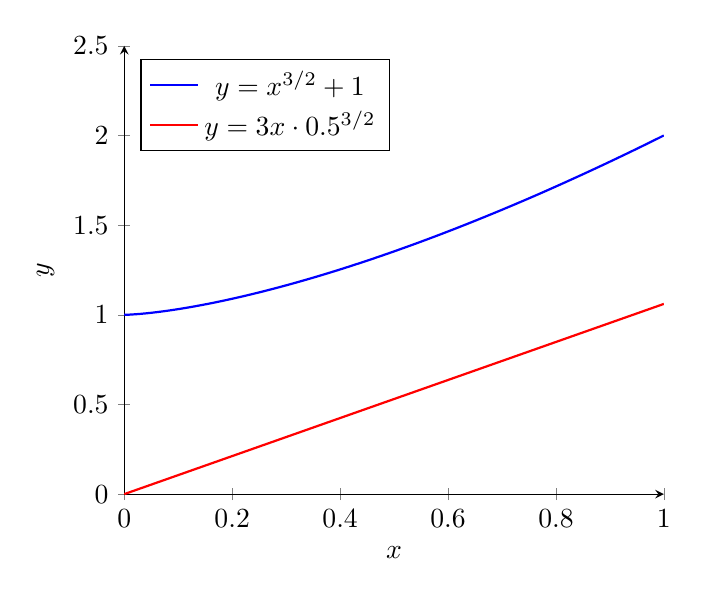
\begin{tikzpicture}
        \begin{axis}[
            axis lines = left,
            xlabel = $x$,
            ylabel = $y$,
            legend pos = north west,
            xmin=0, xmax=1, ymin=0, ymax=2.5,
            samples=100,
            domain=0:1
        ]
            % Plot y = x^(3/2) + 1
            \addplot[blue, thick] {x^(3/2) + 1};
            \addlegendentry{$y = x^{3/2} + 1$}
            
            % Plot y = 3x * 0.5^(3/2)
            \addplot[red, thick] {3*x*0.5^(3/2)};
            \addlegendentry{$y = 3x \cdot 0.5^{3/2}$}
        \end{axis}
    \end{tikzpicture}
    \caption{Comparison of $y = x^{3/2} + 1$ and $y = 3x \cdot 0.5^{3/2}$}
    \label{fig:comparison}
\end{figure}
\section*{5}


\end{document}